
%----------------------------------------------------------------------------------------
%	PACKAGES AND OTHER DOCUMENT CONFIGURATIONS
%----------------------------------------------------------------------------------------

\documentclass{article}


%----------------------------------------------------------------------------------------
%	PACKAGES AND OTHER DOCUMENT CONFIGURATIONS
%----------------------------------------------------------------------------------------

\usepackage{amsmath,amsfonts,stmaryrd,amssymb} % Math packages

\usepackage{enumerate} % Custom item numbers for enumerations
\usepackage{subcaption}
\usepackage[ruled]{algorithm2e} % Algorithms
\usepackage{graphicx}
\usepackage[framemethod=tikz]{mdframed} % Allows defining custom boxed/framed environments

\usepackage{listings} % File listings, with syntax highlighting
\lstset{
	basicstyle=\ttfamily, % Typeset listings in monospace font
}

%----------------------------------------------------------------------------------------
%	DOCUMENT MARGINS
%----------------------------------------------------------------------------------------

\usepackage{geometry} % Required for adjusting page dimensions and margins

\geometry{
	paper=a4paper, % Paper size, change to letterpaper for US letter size
	top=2.5cm, % Top margin
	bottom=3cm, % Bottom margin
	left=2.5cm, % Left margin
	right=2.5cm, % Right margin
	headheight=14pt, % Header height
	footskip=1.5cm, % Space from the bottom margin to the baseline of the footer
	headsep=1.2cm, % Space from the top margin to the baseline of the header
	%showframe, % Uncomment to show how the type block is set on the page
}

%----------------------------------------------------------------------------------------
%	FONTS
%----------------------------------------------------------------------------------------
\usepackage[english, greek]{babel}
\usepackage[utf8]{inputenc} % Required for inputting international characters
\usepackage[T1]{fontenc} % Output font encoding for international characters
\newcommand{\eng}[1]{{\selectlanguage{english}#1}}
\newcommand{\gre}[1]{{\selectlanguage{greek}#1}}

%\usepackage{XCharter} % Use the XCharter fonts

%----------------------------------------------------------------------------------------
%	COMMAND LINE ENVIRONMENT
%----------------------------------------------------------------------------------------

% Usage:
% \begin{commandline}
%	\begin{verbatim}
%		$ ls
%		
%		Applications	Desktop	...
%	\end{verbatim}
% \end{commandline}

\mdfdefinestyle{commandline}{
	leftmargin=10pt,
	rightmargin=10pt,
	innerleftmargin=15pt,
	middlelinecolor=black!50!white,
	middlelinewidth=2pt,
	frametitlerule=false,
	backgroundcolor=black!5!white,
	frametitle={Command Line},
	frametitlefont={\normalfont\sffamily\color{white}\hspace{-1em}},
	frametitlebackgroundcolor=black!50!white,
	nobreak,
}

% Define a custom environment for command-line snapshots
\newenvironment{commandline}{
	\medskip
	\begin{mdframed}[style=commandline]
}{
	\end{mdframed}
	\medskip
}

%----------------------------------------------------------------------------------------
%	FILE CONTENTS ENVIRONMENT
%----------------------------------------------------------------------------------------

% Usage:
% \begin{file}[optional filename, defaults to "File"]
%	File contents, for example, with a listings environment
% \end{file}

\mdfdefinestyle{file}{
	innertopmargin=1.6\baselineskip,
	innerbottommargin=0.8\baselineskip,
	topline=false, bottomline=false,
	leftline=false, rightline=false,
	leftmargin=2cm,
	rightmargin=2cm,
	singleextra={%
		\draw[fill=black!10!white](P)++(0,-1.2em)rectangle(P-|O);
		\node[anchor=north west]
		at(P-|O){\ttfamily\mdfilename};
		%
		\def\l{3em}
		\draw(O-|P)++(-\l,0)--++(\l,\l)--(P)--(P-|O)--(O)--cycle;
		\draw(O-|P)++(-\l,0)--++(0,\l)--++(\l,0);
	},
	nobreak,
}

% Define a custom environment for file contents
\newenvironment{file}[1][File]{ % Set the default filename to "File"
	\medskip
	\newcommand{\mdfilename}{#1}
	\begin{mdframed}[style=file]
}{
	\end{mdframed}
	\medskip
}

%----------------------------------------------------------------------------------------
%	NUMBERED QUESTIONS ENVIRONMENT
%----------------------------------------------------------------------------------------

% Usage:
% \begin{question}[optional title]
%	Question contents
% \end{question}

\mdfdefinestyle{question}{
	innertopmargin=1.2\baselineskip,
	innerbottommargin=0.8\baselineskip,
	roundcorner=5pt,
	nobreak,
	singleextra={%
		\draw(P-|O)node[xshift=1em,anchor=west,fill=white,draw,rounded corners=5pt]{%
		Question \theQuestion\questionTitle};
	},
}

\newcounter{Question} % Stores the current question number that gets iterated with each new question

% Define a custom environment for numbered questions
\newenvironment{question}[1][\unskip]{
	\bigskip
	\stepcounter{Question}
	\newcommand{\questionTitle}{~#1}
	\begin{mdframed}[style=question]
}{
	\end{mdframed}
	\medskip
}

%----------------------------------------------------------------------------------------
%	WARNING TEXT ENVIRONMENT
%----------------------------------------------------------------------------------------

% Usage:
% \begin{warn}[optional title, defaults to "Warning:"]
%	Contents
% \end{warn}

\mdfdefinestyle{warning}{
	topline=false, bottomline=false,
	leftline=false, rightline=false,
	nobreak,
	singleextra={%
		\draw(P-|O)++(-0.5em,0)node(tmp1){};
		\draw(P-|O)++(0.5em,0)node(tmp2){};
		\fill[black,rotate around={45:(P-|O)}](tmp1)rectangle(tmp2);
		\node at(P-|O){\color{white}\scriptsize\bf !};
		\draw[very thick](P-|O)++(0,-1em)--(O);%--(O-|P);
	}
}

% Define a custom environment for warning text
\newenvironment{warn}[1][Warning:]{ % Set the default warning to "Warning:"
	\medskip
	\begin{mdframed}[style=warning]
		\noindent{\textbf{#1}}
}{
	\end{mdframed}
}

%----------------------------------------------------------------------------------------
%	INFORMATION ENVIRONMENT
%----------------------------------------------------------------------------------------

% Usage:
% \begin{info}[optional title, defaults to "Info:"]
% 	contents
% 	\end{info}

\mdfdefinestyle{info}{%
	topline=false, bottomline=false,
	leftline=false, rightline=false,
	nobreak,
	singleextra={%
		\fill[black](P-|O)circle[radius=0.4em];
		\node at(P-|O){\color{white}\scriptsize\bf i};
		\draw[very thick](P-|O)++(0,-0.8em)--(O);%--(O-|P);
	}
}

% Define a custom environment for information
\newenvironment{info}[1][Info:]{ % Set the default title to "Info:"
	\medskip
	\begin{mdframed}[style=info]
		\noindent{\textbf{#1}}
}{
	\end{mdframed}
}
 % Include the file specifying the document structure and custom commands

%----------------------------------------------------------------------------------------
%	ASSIGNMENT INFORMATION
%----------------------------------------------------------------------------------------

\title{Αρχιτεκτονική Παράλληλων και Κατανεμημένων Υπολογιστών} % Title of the assignment

\author{Άρης Ζερβάκης - Στέφανος Καλογεράκης} % Author name and email address

\date{Πολυτεχνείο Κρήτης --- \today} % University, school and/or department name(s) and a date

%----------------------------------------------------------------------------------------

\begin{document}

\maketitle % Print the title

%----------------------------------------------------------------------------------------
%	INTRODUCTION
%----------------------------------------------------------------------------------------

\section*{Εισαγωγή} % Unnumbered section
Στη δεύτερη εργαστηριακή άσκηση καλεστήκαμε να χρησιμοποιήσουμε συνδιαστικά \eng{Streaming SIMD Extensions (SSE), MPI} και \eng{Pthreads} με σκοπό την παραλληλοποίηση του υπολογισμού του ω \eng{statistic}, το οποίο εφαρμόζεται για ανίχνευση θετικής επιλογής σε ακολουθίες \eng{DNA}. Ως κώδικας αναφοράς, χρησιμοποιήθηκε που δόθηκε απο τον διδάσκοντα του μαθήματος (φάκελος με όνομα \eng{Serial}).\\
\begin{warn}[] % Information block
	Για την υλοποίηση της άσκησης μας προχωρήσαμε σε 4 διαφορετικές υλοποιήσεις:\\
    1. Παραλληλοποίηση με \eng{SSE} Εντολές\\
    2. Παραλληλοποίηση με \eng{SSE} Εντολές και \eng{Pthreads}\\
    3. Παραλληλοποίηση με \eng{SSE} Εντολές και \eng{Pthreads} και \eng{MPI}\\
    4. (\eng{Bonus}) Παραλληλοποίηση με \eng{SSE} Εντολές για διαφορετικά \eng{Memory Layout}
\end{warn}

%----------------------------------------------------------------------------------------
%	Υλοποίηση
%----------------------------------------------------------------------------------------

\section{Υλοποίηση} % Numbered section
Για τον σειριακό υπολογισμό του ω \eng{statistic}, χρησιμοποιήσαμε αυτούσιο τον \eng{reference code}χωρίς να πραγματοποίησουμε αλλαγές και για αυτό δεν γίνεται κάποια παραπάνω αναφορά. Παρακάτω γίνεται ανάλυση όλων των μεθόδων παραλληλοποίησης που μελετήθηκαν στα πλαίσια αυτού του πρότζεκτ.\\

\subsection{\eng{SSE} Εντολές}

Η μέθοδος παραλληλοποίησης με τη χρήση \eng{SSE} εντολών υλοποιήθηκε με τη χρήση \eng{pointers} όπως είδαμε και στις διαλέξεις. Αξίζει να σχολιάσουμε ότι επιλέξαμε την συγκεκριμένη μέθοδο σε σύγκριση με την υλοποίηση με χρήση \eng{load} καθώς όπως διδαχτήκαμε είναι πιο γρήγορη. Μετά από δοκιμή στα δικά μας δεδομένα-υπολογισμούς επιβεβαιώσαμε το συγκεκριμένο γεγονός αφού η χρήση των \eng{pointers} οδήγησε σε λίγο πιο γρήγορο χρόνο εκτέλεσης που είναι και βασικό ζητούμενο της παραλληλοποίησης.\\
\newline
-Όλες οι μεταβλητές οι οποίες ξεκινούν με \eng{underscore} συσχετίζονται με το λειτουργικό κομμάτι της \eng{SSE} υλοποίησης.\\
-Δημιουργήθηκαν οι παρακάτω μεταβλητές πλάτους 128 \eng{bits}.
\selectlanguage{english}
% File contents

\begin{lstlisting}
 __m128 *mVec_ptr = (__m128 *) mVec;
 __m128 *nVec_ptr = (__m128 *) nVec;
 __m128 *LVec_ptr = (__m128 *) LVec;
 __m128 *RVec_ptr = (__m128 *) RVec;
 __m128 *CVec_ptr = (__m128 *) CVec;
 __m128 *FVec_ptr = (__m128 *) FVec;

 __m128 avgF_vec = _mm_setzero_ps();
 __m128 maxF_vec = _mm_setzero_ps();
 __m128 minF_vec = _mm_set_ps1(FLT_MAX);
\end{lstlisting}

\selectlanguage{greek}

Για την υλοποίηση των υπολογισμών έγιναν οι παρακάτω αλλαγές:\\
-Αλλαγή των \eng{malloc}, \eng{free} με τις \textunderscore \textunderscore \eng{mm}\textunderscore \eng{malloc}, \textunderscore \textunderscore \eng{mm}\textunderscore \eng{free}. 
(εντολές που χρησιμοποιούνται για ευθυγράμμιση των δεδομένων).\\
-Tροποποίηση εντολών.
(Σε σχόλια παρατίθενται οι εντολές στην αρχική μορφή τους και έπειτα η τροποποίηση τους)
\newline
\selectlanguage{english}
\begin{lstlisting}
for(unsigned int i=0; i<N/4 ;i++){

            //float num_0 = LVec[i] + RVec[i];
            temp_num_0 = _mm_add_ps(LVec_ptr[i],RVec_ptr[i]);

            //float num_1 = mVec[i]*(mVec[i]-1.0f)/2.0f;
            temp_num_1 = _mm_sub_ps(mVec_ptr[i], temp_one);
            temp_num_1 = _mm_mul_ps(mVec_ptr[i], temp_num_1);
            temp_num_1 = _mm_div_ps(temp_num_1, temp_two);

            //float num_2 = nVec[i]*(nVec[i]-1.0f)/2.0f;
            temp_num_2 = _mm_sub_ps(nVec_ptr[i], temp_one);
            temp_num_2 = _mm_mul_ps(nVec_ptr[i], temp_num_2);
            temp_num_2 = _mm_div_ps(temp_num_2, temp_two);

            //float num = num_0/(num_1+num_2);
            temp_num = _mm_add_ps(temp_num_1,temp_num_2);
            temp_num = _mm_div_ps(temp_num_0, temp_num);

            //float den_0 = CVec[i]-LVec[i]-RVec[i];
            temp_den_0 = _mm_sub_ps(CVec_ptr[i], LVec_ptr[i]);
            temp_den_0 = _mm_sub_ps(temp_den_0, RVec_ptr[i]);

            //float den_1 = mVec[i]*nVec[i];
            temp_den_1 = _mm_mul_ps(mVec_ptr[i], nVec_ptr[i]);

            //float den = den_0/den_1;
            temp_den = _mm_div_ps(temp_den_0, temp_den_1);

            //FVec[i] = num/(den+0.01f);
            FVec_ptr[i] = _mm_add_ps(temp_den, __temp_one);
            FVec_ptr[i] = _mm_div_ps(temp_num, FVec_ptr[i]);

            //maxF = FVec[i]>maxF?FVec[i]:maxF;
            maxF_vec = _mm_max_ps(FVec_ptr[i], maxF_vec);

            //minF = FVec[i]<minF?FVec[i]:minF;
            minF_vec = _mm_min_ps(FVec_ptr[i], minF_vec);

            //avgF += FVec[i];
            avgF_vec = _mm_add_ps(FVec_ptr[i], avgF_vec );
}
\end{lstlisting}
\selectlanguage{greek}
\vspace{5mm}
Στην υλοποίηση πραγματοποιούμε \eng{loop unrolling} και \eng{jamming} στις εντολές του \eng{for-loop}, με κάθε \eng{i} να αναλογεί σε 4 στοιχεία. ΄Οσον αφορα την εύρεση του \eng{max, min, avg} έχοντας ορίσει τις κατάλληλες \eng{m128} μεταβλητές πραγματοποιύμε επιμέρους σε συγκρίσεις ανά τετράδες με \eng{SSE} εντολές και στο τέλος αποθηκεύουμε σε μια \eng{global} μεταβλητή την σωστή τιμή ανάλογα με την περίπτωση.\\
\newpage
\selectlanguage{english}
\begin{lstlisting}
maxF = maxF_vec[0];
maxF = maxCalc(maxF_vec[1],maxF);
maxF = maxCalc(maxF_vec[2],maxF);
maxF = maxCalc(maxF_vec[3],maxF);

minF = minF_vec[0];
minF = minCalc(minF_vec[1],minF);
minF = minCalc(minF_vec[2],minF);
minF = minCalc(minF_vec[3],minF);

avgF = avgF_vec[0] + avgF_vec[1] + avgF_vec[2] + avgF_vec[3];
\end{lstlisting}
\selectlanguage{greek}
\vspace{5mm}
Στο τέλος, προσθέσαμε ένα κομμάτι κώδικα το οποίο για τα συγκεκριμένα δεδομένα που δοκιμάζουμε δεν πρόκειται να χρησιμοποιηθεί αλλά εισάγεται για λόγους πληρότητας, σε περίπτωση που υπάρξει ανάγκη για δοκιμή σε άλλα δεδομένα.

\selectlanguage{english}
\begin{lstlisting}
for (int j = (N - N % 4); j < N; j++) {
            float num_0 = LVec[j] + RVec[j];
            float num_1 = mVec[j] * (mVec[j] - 1.0f) / 2.0f;
            float num_2 = nVec[j] * (nVec[j] - 1.0f) / 2.0f;
            float num = num_0 / (num_1 + num_2);
            float den_0 = CVec[j] - LVec[j] - RVec[j];
            float den_1 = mVec[j] * nVec[j];
            float den = den_0 / den_1;

            FVec[j] = num / (den + 0.01f);
            maxF = FVec[j] > maxF ? FVec[j] : maxF;
            minF = FVec[j]<minF?FVec[j]:minF;
            avgF += FVec[j];
}
\end{lstlisting}
\selectlanguage{greek}
%------------------------------------------------

\subsection{\eng{SSE} Εντολές και \eng{Pthreads} }

Στο δέυτερο μέρος έπρεπε να παραλληλοποιήσουμε το \eng{reference code} συνδιαστικά, με \eng{SSE} Εντολές και \eng{Pthreads}. 
Τα \eng{Pthreads} δημιουργούνται στην αρχή της \eng{main} και γίνονται \eng{join} πριν την επιστροφή της. Στην υλοποίηση μας όσο το \eng{master thread} αρχικοποιεί τις μεταβλητές μας, τα \eng{worker threads} είναι σε κατάσταση \eng{busy wait} και έπειτα σε κάθε \eng{iteration} του \eng{for-loop} το \eng{master} μοιράζει στα \eng{worker threads} τους υπολογισμούς. Ο συγχρονισμός των \eng{Pthreads} σε κάθε \eng{iteration} επιτυγχάνεται με τη χρήση \eng{barrier}.


\subsection{\eng{SSE} Εντολές, \eng{Pthreads} και \eng{MPI} }

In malesuada ullamcorper urna, sed dapibus diam sollicitudin non. Donec elit odio, accumsan ac nisl a, tempor imperdiet eros. Donec porta tortor eu risus consequat, a pharetra tortor tristique. Morbi sit amet laoreet erat. Morbi et luctus diam, quis porta ipsum. Quisque libero dolor, suscipit id facilisis eget, sodales volutpat dolor. Nullam vulputate interdum aliquam. Mauris id convallis erat, ut vehicula neque. Sed auctor nibh et elit fringilla, nec ultricies dui sollicitudin. Vestibulum vestibulum luctus metus venenatis facilisis. Suspendisse iaculis augue at vehicula ornare. Sed vel eros ut velit fermentum porttitor sed sed massa. Fusce venenatis, metus a rutrum sagittis, enim ex maximus velit, id semper nisi velit eu purus.

\newpage
\subsection{\eng{BONUS}: Υλοποίηση διαφορετικών \eng{memory layout} για τη βελτιστοποίηση της παραλληλοποίησης με \eng{SSE} Εντολές }

In malesuada ullamcorper urna, sed dapibus diam sollicitudin non. Donec elit odio, accumsan ac nisl a, tempor imperdiet eros. Donec porta tortor eu risus consequat, a pharetra tortor tristique. Morbi sit amet laoreet erat. Morbi et luctus diam, quis porta ipsum. Quisque libero dolor, suscipit id facilisis eget, sodales volutpat dolor. Nullam vulputate interdum aliquam. Mauris id convallis erat, ut vehicula neque. Sed auctor nibh et elit fringilla, nec ultricies dui sollicitudin. Vestibulum vestibulum luctus metus venenatis facilisis. Suspendisse iaculis augue at vehicula ornare. Sed vel eros ut velit fermentum porttitor sed sed massa. Fusce venenatis, metus a rutrum sagittis, enim ex maximus velit, id semper nisi velit eu purus.

\begin{figure}[h!]
\centering
  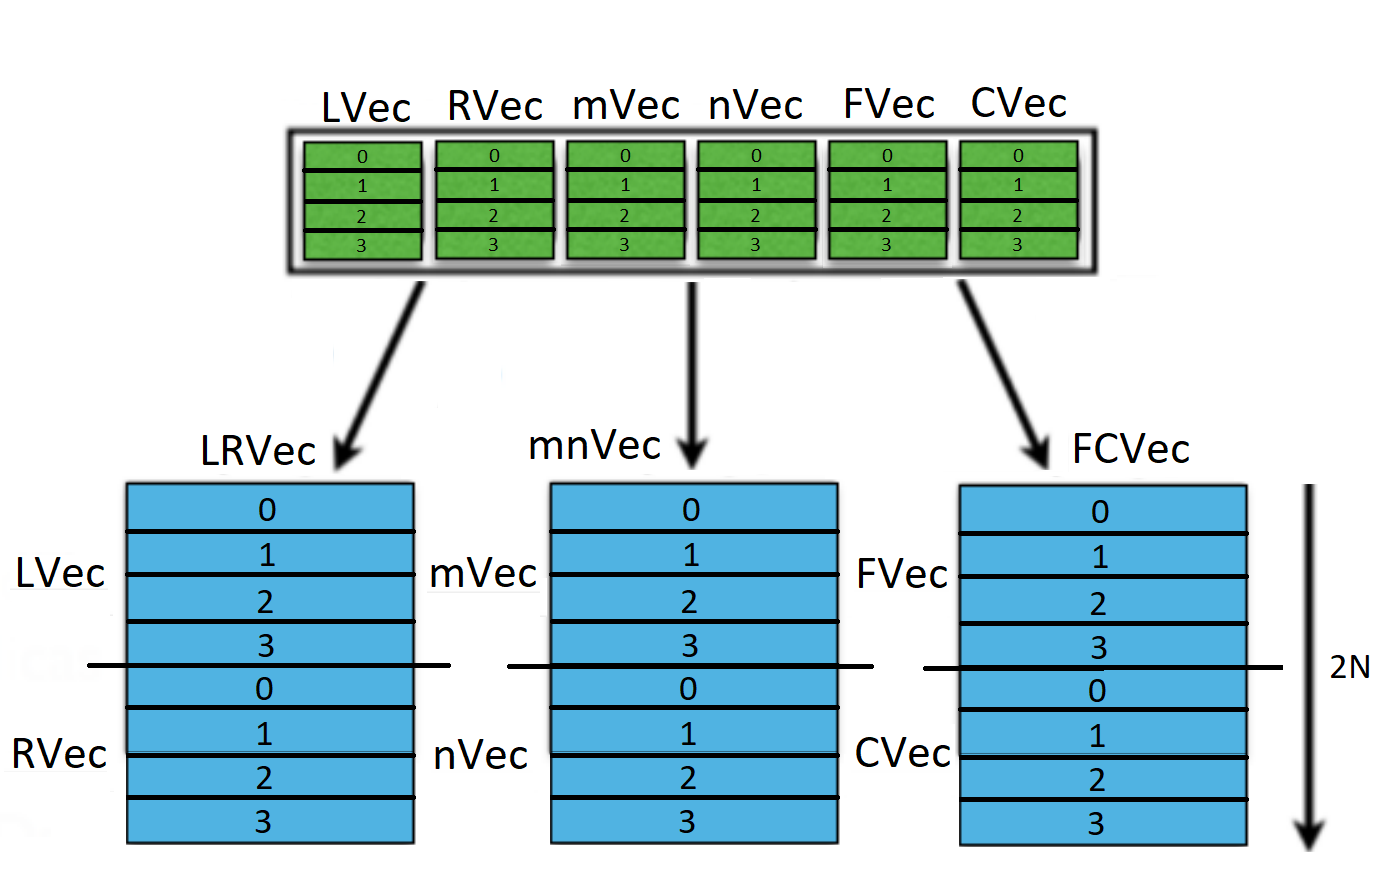
\includegraphics[width=0.8\linewidth]{SCHEME.png}
  \caption{\eng{Comment}}
\end{figure}
%----------------------------------------------------------------------------------------
%----------------------------------------------------------------------------------------
\newpage
\section{Εκτέλεση}

Για την εκτέλεση, απλά καλούμαστε να τρέξουμε στο \eng{command line} την παρακάτω εντολή, παίρνοντας τα ακόλουθα
αποτελέσματα:
\vspace{10mm}
\selectlanguage{english}
% Command-line "screenshot"
\begin{commandline}
	\begin{verbatim}
$ ./run.sh

---------------------- Building everything ------------------------------


---------------------- Giving permissions -------------------------------


---------------------- Reference Code N:10000000-------------------------
Omega time 0.177147s - Total time 2.829882s - Min -2.711918e+06 - 
Max 6.048419e+05 - Avg -6.529043e-01



---------------------- SSE N:10000000------------------------------------
Omega time 0.106534s - Total time 2.149127s - Min -2.711918e+06 - 
Max 6.048419e+05 - Avg -6.348448e-01



-------------- SSE-PTHREADS N:10000000, PTHREADS:2-----------------------
Omega time 0.053595s - Total time 2.226116s - Min -2.711918e+06 - 
Max 6.048419e+05 - Avg -6.332115e-01


--------------- SSE-PTHREADS N:10000000, PTHREADS:4----------------------
Omega time 0.044613s - Total time 2.552894s - Min -2.711918e+06 - 
Max 6.048419e+05 - Avg -6.323332e-01
      \end{verbatim}
\end{commandline}


\begin{commandline}
      \begin{verbatim}


-------- SSE-PTHREADS-MPI N:10000000, PTHREADS:2, PROCESSES:2------------
Omega time 0.041026s - Total time 2.108915s - Min -2.711918e+06 - 
Max 6.048419e+05 - Avg -6.323332e-01


-------- SSE-PTHREADS-MPI N:10000000, PTHREADS:4, PROCESSES:2------------
Omega time 0.040200s - Total time 4.056555s - Min -2.711918e+06 - 
Max 6.048419e+05 - Avg -6.323262e-01


-------- SSE-PTHREADS-MPI N:10000000, PTHREADS:2, PROCESSES:4------------
Omega time 0.028752s - Total time 4.942250s - Min -2.711918e+06 - 
Max 6.048419e+05 - Avg -6.323262e-01


-------- SSE-PTHREADS-MPI N:10000000, PTHREADS:4, PROCESSES:4------------
Omega time 0.033914s - Total time 8.615657s - Min -2.711918e+06 - 
Max 6.048419e+05 - Avg -6.321101e-01


----------------------- Bonus -------------------------------------------


---------------------- SSE N:10000000(AGAIN)-----------------------------
Omega time 0.108413s - Total time 2.189199s - Min -2.711918e+06 - 
Max 6.048419e+05 - Avg -6.348448e-01


------------ SSE N:10000000, SSE_MEM_LAYOUT 3 vectors--------------------
Omega time 0.105147s - Total time 2.193838s - Min -2.711918e+06 - 
Max 6.048419e+05 - Avg -6.348448e-01


------------ SSE N:10000000, SSE_MEM_LAYOUT 2 vectors--------------------
Omega time 0.104894s - Total time 2.180221s - Min -2.711918e+06 - 
Max 6.048419e+05 - Avg -6.348448e-01


------------ SSE N:10000000, SSE_MEM_LAYOUT 1 vector --------------------
Omega time 0.104966s - Total time 2.203330s - Min -2.711918e+06 - 
Max 6.048419e+05 - Avg -6.348448e-01

      \end{verbatim}
\end{commandline}

\selectlanguage{greek}
% Warning text, with a custom title
\begin{warn}[Σημείωση:]
  Για να τρέξουμε το \eng{run script} είναι απαραίτητο να βρισκόμαστε στο \eng{directory} όπου έχουμε τοποθετήσει τα αρχεία μας και να έχουμε ήδη εγκατεστημένα το \eng{gcc, make} και \eng{mpich} ώστε να μπορεί να γίνει \eng{compile} και να πάρουμε τα αποτελέσματα.
\end{warn}

%----------------------------------------------------------------------------------------

\section{Συμπεράσματα}

Απεικονίζοντας τους παραπάνω χρόνους μπορούμε να εξάγουμε πολύτιμα συμπεράσματα για τις υλοποιήσεις μας, υπολογίζοντας το \eng{speedup} που έχουμε στην εκάστοτε περίπτωση.\\
Το \eng{speedup} υπολογίζεται με τον ακόλουθο τύπο:

\selectlanguage{english}
\begin{equation}
     Speedup = \dfrac{Serial Code Execution Time}{Parallelized Code Execution Time}
\end{equation}
\selectlanguage{greek}


\subsection{\eng{SSE} Εντολές}

In malesuada ullamcorper urna, sed dapibus diam sollicitudin non. Donec elit odio, accumsan ac nisl a, tempor imperdiet eros. Donec porta tortor eu risus consequat, a pharetra tortor tristique. Morbi sit amet laoreet erat. Morbi et luctus diam, quis porta ipsum. Quisque libero dolor, suscipit id facilisis eget, sodales volutpat dolor. Nullam vulputate interdum aliquam. Mauris id convallis erat, ut vehicula neque. Sed auctor nibh et elit fringilla, nec ultricies dui sollicitudin. Vestibulum vestibulum luctus metus venenatis facilisis. Suspendisse iaculis augue at vehicula ornare. Sed vel eros ut velit fermentum porttitor sed sed massa. Fusce venenatis, metus a rutrum sagittis, enim ex maximus velit, id semper nisi velit eu purus.

\begin{figure}[h!]
\centering
  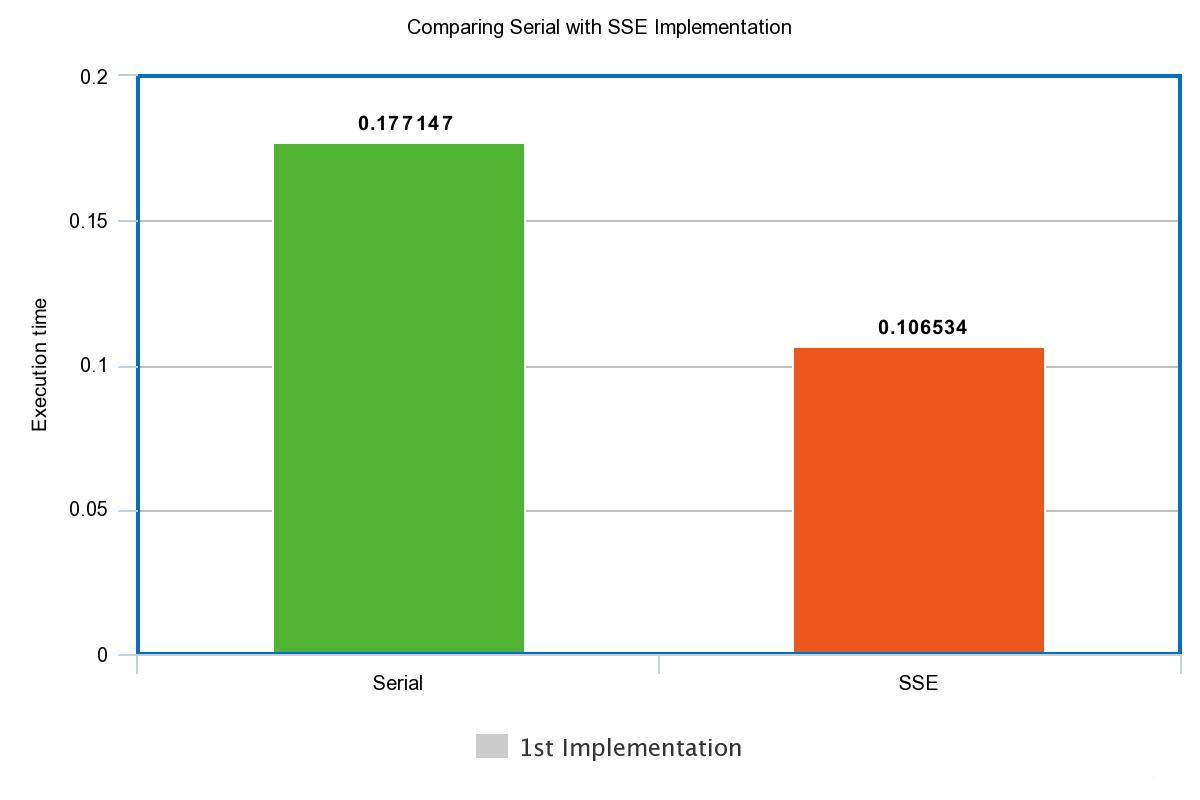
\includegraphics[width=0.8\linewidth]{SSE.jpeg}
  \caption{\eng{Comparing Serial with SSE Implementation}}
\end{figure}

\newpage
\subsection{\eng{SSE} Εντολές, \eng{Pthreads}}

In malesuada ullamcorper urna, sed dapibus diam sollicitudin non. Donec elit odio, accumsan ac nisl a, tempor imperdiet eros. Donec porta tortor eu risus consequat, a pharetra tortor tristique. Morbi sit amet laoreet erat. Morbi et luctus diam, quis porta ipsum. Quisque libero dolor, suscipit id facilisis eget, sodales volutpat dolor. Nullam vulputate interdum aliquam. Mauris id convallis erat, ut vehicula neque. Sed auctor nibh et elit fringilla.

\begin{figure}[h!]
\centering
  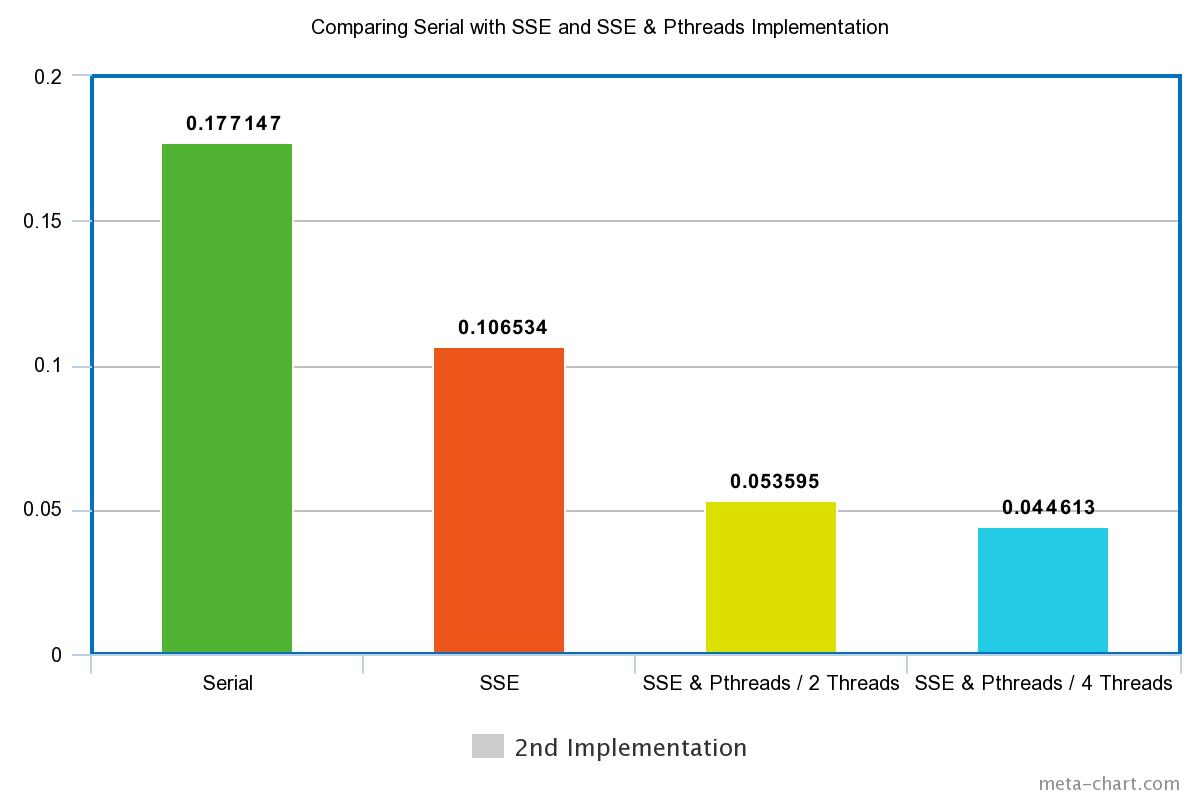
\includegraphics[width=0.8\linewidth]{SSE_PTHREADS.jpeg}
  \caption{\eng{Comparing Serial with SSE and Pthreads Implementation}}
\end{figure}

\newpage
\subsection{\eng{SSE} Εντολές, \eng{Pthreads} και \eng{MPI} }

Στην περίπτωση παραλληλοποίησης του κώδικα με \eng{MPI} δε μας ζητήθηκε να αξιολογήσουμε την απόδοση και το \eng{speedup}. Ακολουθούν ενδεικτικά τα διαγράμματα με τους χρόνους που 
λάβαμε:
\vspace{5mm}
\begin{figure}[h!]
\centering 
  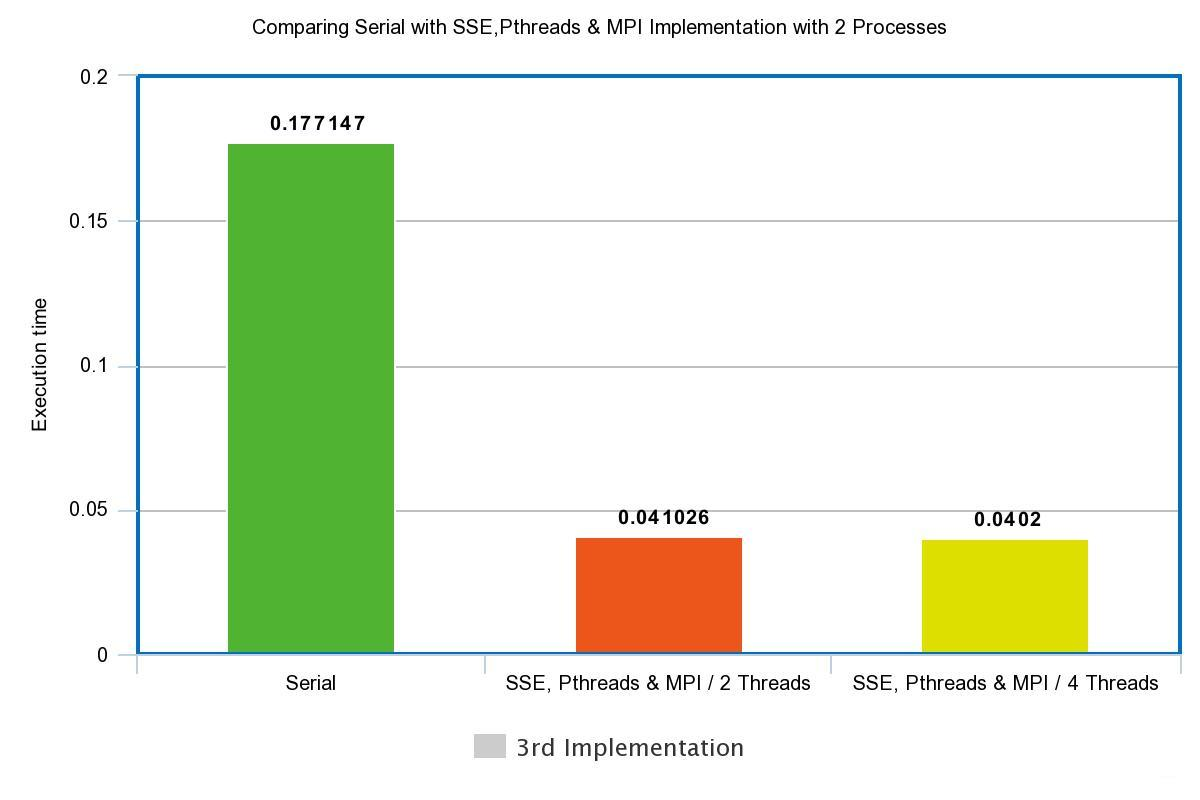
\includegraphics[width=0.8\linewidth]{MPI2.jpeg}
  \caption{\eng{Comparing Serial with SSE,Pthreads and MPI Implementation with 2 Processes} }
\end{figure}

\begin{figure}[h!]
\centering
  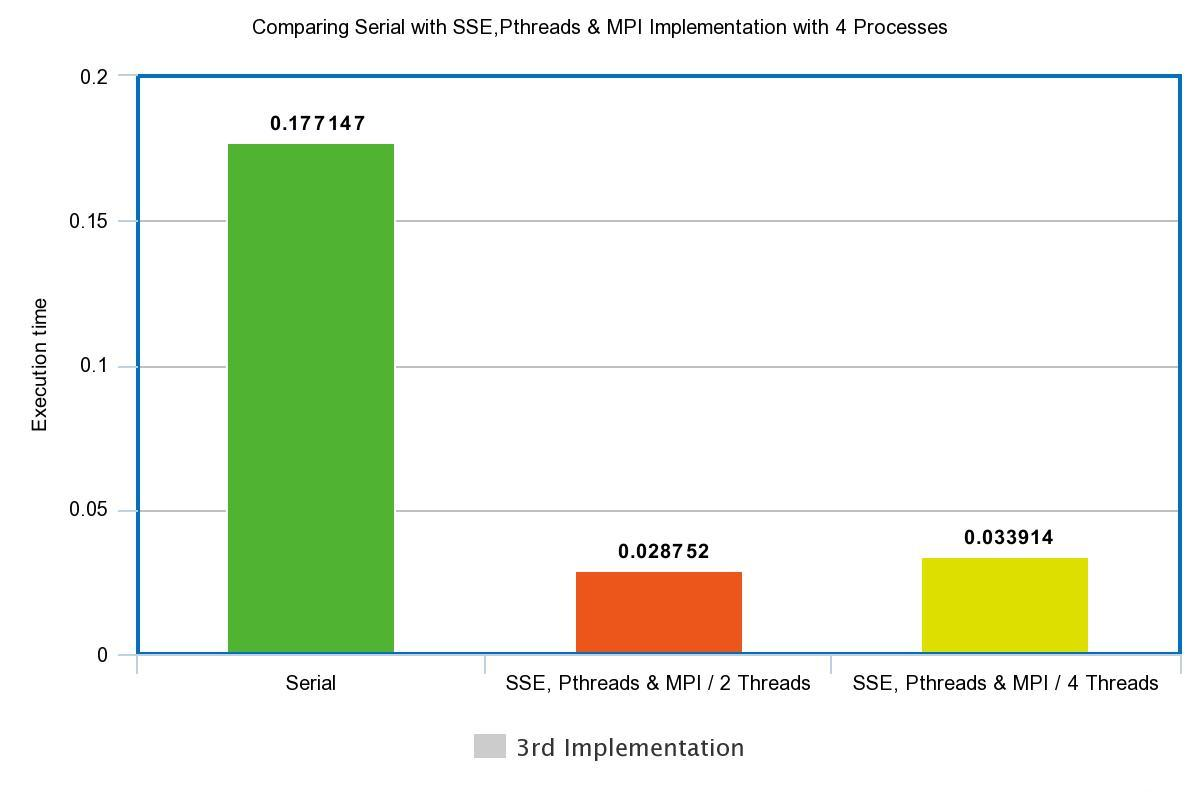
\includegraphics[width=0.8\linewidth]{MPI4.jpeg}
  \caption{\eng{Comparing Serial with SSE,Pthreads and MPI Implementation with 2 Processes} }
\end{figure}

\newpage

\subsection{\eng{BONUS}: \eng{SSE Memory Layouts}}
% Math equation/formula

In malesuada ullamcorper urna, sed dapibus diam sollicitudin non. Donec elit odio, accumsan ac nisl a, tempor imperdiet eros. Donec porta tortor eu risus consequat, a pharetra tortor tristique. Morbi sit amet laoreet erat. Morbi et luctus diam, quis porta ipsum. Quisque libero dolor, suscipit id facilisis eget, sodales volutpat dolor. Nullam vulputate interdum aliquam. Mauris id convallis erat, ut vehicula neque. Sed auctor nibh et elit fringilla, nec ultricies dui sollicitudin. Vestibulum vestibulum luctus metus venenatis facilisis. Suspendisse iaculis augue at vehicula ornare. Sed vel eros ut velit fermentum porttitor sed sed massa. Fusce venenatis, metus a rutrum sagittis, enim ex maximus velit, id semper nisi velit eu purus.

\begin{figure}[h!]
\centering 
  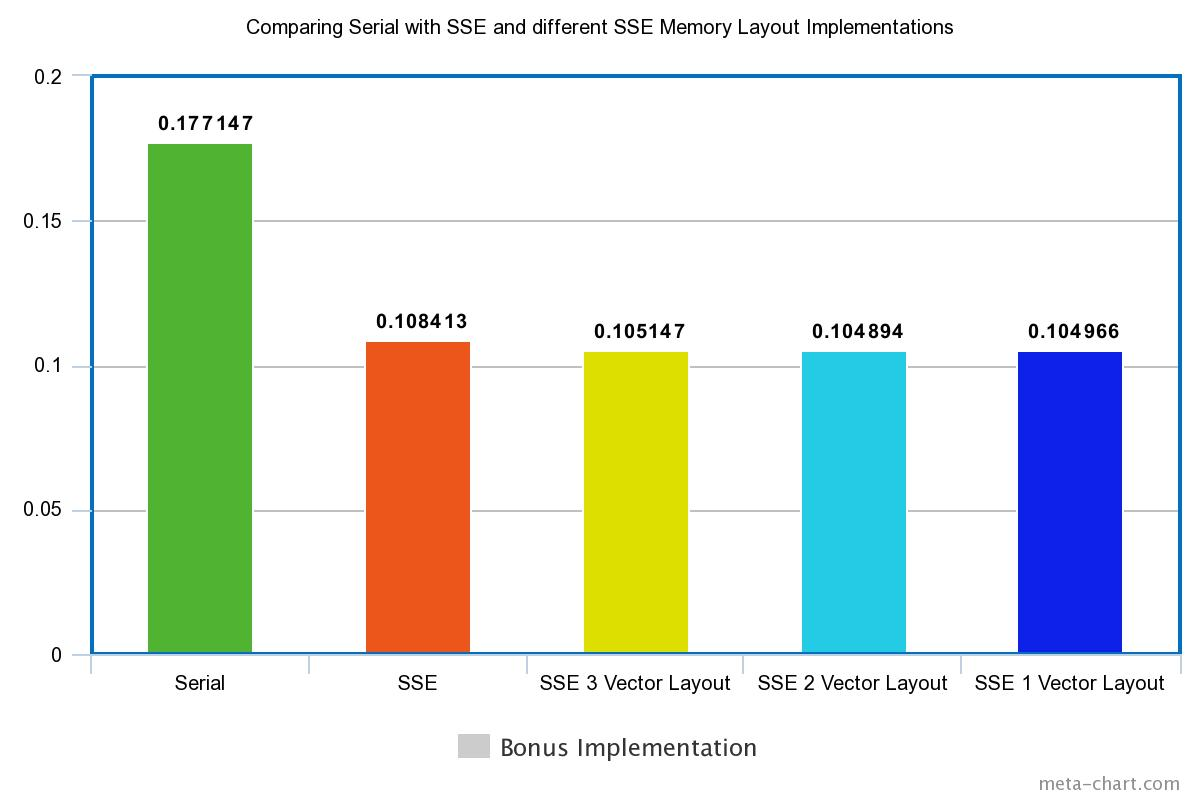
\includegraphics[width=0.8\linewidth]{BONUS.jpeg}
  \caption{\eng{Comparing different SSE Memory Layouts} }
\end{figure}

In malesuada ullamcorper urna, sed dapibus diam sollicitudin non. Donec elit odio, accumsan ac nisl a, tempor imperdiet eros. Donec porta tortor eu risus consequat, a pharetra tortor tristique. Morbi sit amet laoreet erat. Morbi et luctus diam, quis porta ipsum. Quisque libero dolor, suscipit id facilisis eget, sodales volutpat dolor. Nullam vulputate interdum aliquam. Mauris id convallis erat, ut vehicula neque. Sed auctor nibh et elit fringilla, nec ultricies dui sollicitudin. Vestibulum vestibulum luctus metus venenatis facilisis. Suspendisse iaculis augue at vehicula ornare. Sed vel eros ut velit fermentum porttitor sed sed massa. Fusce venenatis, metus a rutrum sagittis, enim ex maximus velit, id semper nisi velit eu purus.







%\begin{equation}
%     I = \int_{a}^{b} f(x) \; \text{d}x.
%\end{equation}
\end{document}
